\documentclass{minimal}

\usepackage{tikz}
\usetikzlibrary{calc, arrows, fit, positioning}
\definecolor{clamped}{RGB}{200,200,200}

\begin{document}
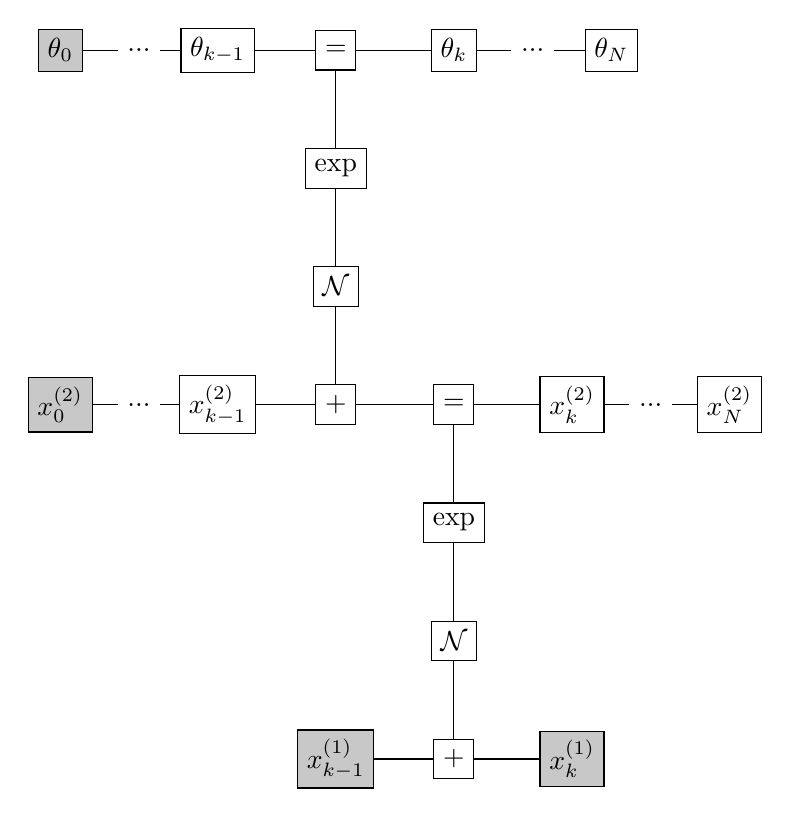
\begin{tikzpicture}
    [
        node distance=15mm,auto,>=latex',
        box/.style={draw, minimum size=.5cm},
        bbox/.style={draw, minimum size=1cm},
        blackbox/.style={draw, fill=black, minimum size=0.25cm}
    ]
    \tikzstyle{line} = [draw, -latex,>=latex]
    \tikzstyle{dash} = [dashed, -latex,>=latex]
    \tikzstyle{branch} = [fill,shape=circle,minimum size=3pt,inner sep=0pt]
    
    \begin{scope}
        % Bottom layer
        \node[box, fill=clamped] (x_l1_k_min) {$x^{(1)}_{k-1}$};
        \node[box, right of=x_l1_k_min] (l1_add) {+};
        \node[box, right of=l1_add, fill=clamped] (x_l1_k) {$x^{(1)}_{k}$};
        \path[line] (x_l1_k_min) edge[-] (l1_add);
        \path[line] (l1_add) edge[-] (x_l1_k);

        % Vertical path from bottom layer upwards
        \node[box, above of=l1_add] (l1_N) {$\mathcal{N}$};
        \node[box, above of=l1_N] (l1_exp) {exp};
        \node[box, above of=l1_exp] (l2_eq) {=};
        \path[line] (l1_add) edge[-] (l1_N);
        \path[line] (l1_N) edge[-] (l1_exp);
        \path[line] (l1_exp) edge[-] (l2_eq);

        % Second layer
        \node[box, right of=l2_eq] (x_l2_k) {$x^{(2)}_{k}$};
        \node[right of=x_l2_k, node distance=1.0cm] (x_l2_N_dots) {...};
        \node[box, right of=x_l2_N_dots, node distance=1.0cm] (x_l2_N) {$x^{(2)}_{N}$};
        \node[box, left of=l2_eq] (l2_add) {+};
        \node[box, left of=l2_add] (x_l2_k_min) {$x^{(2)}_{k-1}$};
        \node[left of=x_l2_k_min, node distance=1.0cm] (x_l2_0_dots) {...};
        \node[box, left of=x_l2_0_dots, node distance=1.0cm, fill=clamped] (x_l2_0) {$x^{(2)}_{0}$};
        \path[line] (x_l2_0) edge[-] (x_l2_0_dots);
        \path[line] (x_l2_0_dots) edge[-] (x_l2_k_min);
        \path[line] (x_l2_k_min) edge[-] (l2_add);
        \path[line] (l2_add) edge[-] (l2_eq);
        \path[line] (l2_eq) edge[-] (x_l2_k);
        \path[line] (x_l2_k) edge[-] (x_l2_N_dots);
        \path[line] (x_l2_N_dots) edge[-] (x_l2_N);

        % Vertical path from second layer upwards
        \node[box, above of=l2_add] (l2_N) {$\mathcal{N}$};
        \node[box, above of=l2_N] (l2_exp) {exp};
        \node[box, above of=l2_exp] (l3_eq) {=};
        \path[line] (l2_add) edge[-] (l2_N);
        \path[line] (l2_N) edge[-] (l2_exp);
        \path[line] (l2_exp) edge[-] (l3_eq);

        % Top layer
        \node[box, right of=l3_eq] (theta_k) {$\theta_{k}$};
        \node[right of=theta_k, node distance=1.0cm] (theta_N_dots) {...};
        \node[box, right of=theta_N_dots, node distance=1.0cm] (theta_N) {$\theta_{N}$};
        \node[box, left of=l3_eq] (theta_k_min) {$\theta_{k-1}$};
        \node[left of=theta_k_min, node distance=1.0cm] (theta_0_dots) {...};
        \node[box, left of=theta_0_dots, node distance=1.0cm, fill=clamped] (theta_0) {$\theta_{0}$};
        \path[line] (theta_0) edge[-] (theta_0_dots);
        \path[line] (theta_0_dots) edge[-] (theta_k_min);
        \path[line] (theta_k_min) edge[-] (l3_eq);
        \path[line] (l3_eq) edge[-] (theta_k);
        \path[line] (theta_k) edge[-] (theta_N_dots);
        \path[line] (theta_N_dots) edge[-] (theta_N);

    \end{scope}
\end{tikzpicture}
\end{document}